
\documentclass[conference]{IEEEtran}

\usepackage{amsmath,amssymb}
\usepackage{graphicx}
\usepackage{booktabs}
\usepackage{tikz}
\usetikzlibrary{arrows.meta,positioning,calc}

% ---- Figure helper: draws PNG if present, otherwise a labelled placeholder ----
\newcommand{\figbox}[2]{\IfFileExists{figures/#1.png}%
  {\includegraphics[width=\linewidth]{figures/#1.png}}%
  {\fbox{\parbox[c][#2][c]{0.92\linewidth}{\centering\footnotesize
   PLACEHOLDER: \detokenize{figures/#1.png} not found}}}}

\newcommand{\Tp}{T_p}
\newcommand{\Kp}{K_p}
\newcommand{\Kv}{K_v}
\newcommand{\vect}[1]{\mathbf{#1}}

\begin{document}

\title{Predictive Tracking and Turret Elevation Control for a Maneuvering Aerial Target with Noisy, Intermittent Radar}

\author{\IEEEauthorblockN{Vanshika Nalamasa}
    Roll Number : 24B2106
\IEEEauthorblockA{Department of Mechanical Engineering\\
Indian Institute of Technology Bombay\\
Mumbai, India\\
}}

\maketitle

\begin{abstract}
This report presents a predictive-feedback design for the elevation axis of a laser turret that must engage a maneuvering aerial target using 20~Hz range and elevation radar with noise and a possible measurement blackout. An extended Kalman filter (EKF) with a constant-acceleration model estimates the target state, which is extrapolated over the 0.5~s prediction horizon and converted to a reference elevation. A proportional gain $\Kp = 1/(\Tp \Kv)$, derived from the turret transfer function, makes the loop's ramp-tracking lag equal to the prediction horizon. The laser is fired by a separate, uncertainty-aware gate. In our own simulations the design obtained at least one hit in each of three standardized scenarios (first hit at 2.70, 4.20 and 4.13~s), but pointing accuracy degrades during maneuvering. Voltage and current saturation are not modelled. The instructor's final evaluation has not yet been run.
\end{abstract}

\begin{IEEEkeywords}
fire control, extended Kalman filter, target prediction, proportional control, radar measurement loss
\end{IEEEkeywords}

%=====================================================================
\section{Introduction}

A fire-control system must aim at where the target \emph{will be} when the weapon acts, not where it was last measured. Here, a radar co-located with the turret reports range and elevation of a target at 20~Hz, with standard deviations $\sigma_r = 1$~m and $\sigma_\theta = 0.02^\circ$, and may lose the target for up to 0.5~s after $t = 1$~s \cite{assign}. Velocity and acceleration are not measured, so they must be inferred from noisy polar data, and differentiating raw measurements would amplify the noise. Moreover, the turret is a third-order electromechanical system whose elevation response lags its command, so even a perfect estimate of the present target position would produce an aim that trails the target. The turret must therefore track a \emph{predicted} elevation $\theta(t+\Tp)$, with $\Tp = 0.5$~s, rather than the measured one.

The design is evaluated in three standardized 10~s scenarios \cite{assign}: (A) non-maneuvering target, (B) a bounded maneuver in both $x$ and $y$ starting at $t=1$~s, and (C) the same maneuver as B with a 0.5~s radar blackout from $t=1.0$~s. The objective is a single, untuned estimator--predictor--controller that keeps the beam within $R_\mathrm{eng}=2$~m of the target at the firing instants, with at least 1~s between pulses. Section~\ref{sec:final} states what has and has not been verified. The source code and scripts are at 
[https://github.com/VanshikaNalamasa/ME319-Assignment-2].

%=====================================================================
\section{System Architecture and Design}

Fig.~\ref{fig:arch} shows the implemented information flow, and Fig.~\ref{fig:geom} the geometry. Radar outputs $(r_m,\theta_m,\text{valid})$ enter an EKF that propagates the state at every controller call and corrects it only when a new valid measurement arrives. The predictor extrapolates the estimate by $\Tp$ using the same motion model and converts the predicted position to an elevation. After clamping to the turret limits this becomes $\theta_\mathrm{ref}$, and the LTI compensator $G_c(s)=\Kp$ forms $V_m=\Kp(\theta_\mathrm{ref}-\theta_\mathrm{turret})$.

\begin{figure*}[t]
\centering
\resizebox{\textwidth}{!}{%
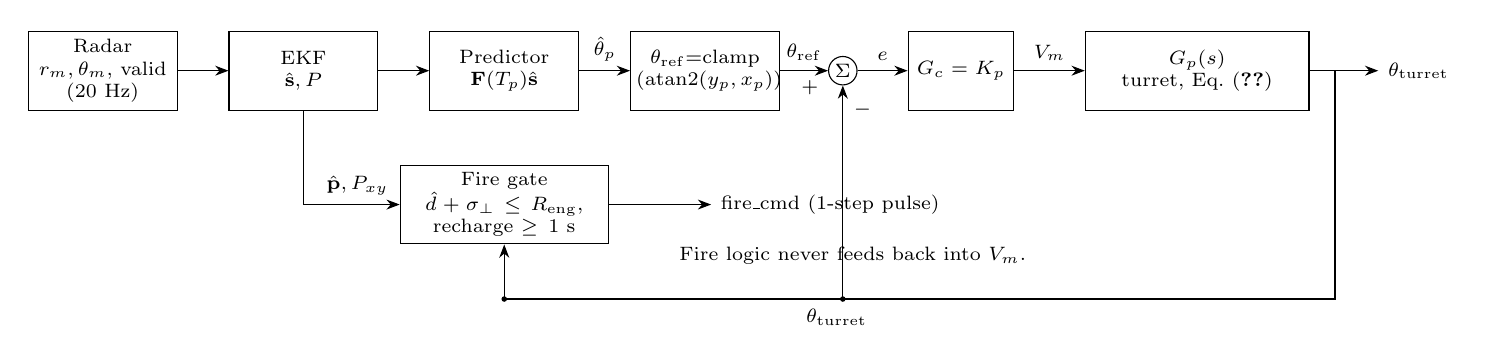
\begin{tikzpicture}[>=Stealth,
  blk/.style={draw,rectangle,minimum height=1.0cm,text width=1.75cm,align=center,font=\scriptsize,inner sep=2pt},
  x=1cm,y=1cm]
\node[blk] (radar) at (0,0) {Radar\\$r_m,\theta_m$, valid\\(20 Hz)};
\node[blk] (ekf)   at (2.55,0) {EKF\\$\hat{\vect s},P$};
\node[blk] (pred)  at (5.1,0) {Predictor\\$\vect F(\Tp)\hat{\vect s}$};
\node[blk] (ref)   at (7.65,0) {$\theta_\mathrm{ref}$=clamp\\$(\mathrm{atan2}(y_p,x_p))$};
\node[circle,draw,inner sep=1pt,font=\scriptsize] (sum) at (9.4,0) {$\Sigma$};
\node[blk,text width=1.2cm] (kp) at (10.9,0) {$G_c=\Kp$};
\node[blk,text width=2.7cm] (plant) at (13.9,0) {$G_p(s)$\\turret, Eq.~\eqref{eq:Gp}};
\node[blk,text width=2.5cm] (fire) at (5.1,-1.7) {Fire gate\\$\hat d+\sigma_\perp\le R_\mathrm{eng}$,\\recharge $\ge1$ s};
\draw[->] (radar) -- (ekf);
\draw[->] (ekf) -- (pred);
\draw[->] (pred) -- node[above,font=\scriptsize]{$\hat\theta_p$} (ref);
\draw[->] (ref) -- node[above,font=\scriptsize]{$\theta_\mathrm{ref}$} (sum);
\draw[->] (sum) -- node[above,font=\scriptsize]{$e$} (kp);
\draw[->] (kp) -- node[above,font=\scriptsize]{$V_m$} (plant);
\coordinate (tap) at (15.65,0);
\draw[->] (plant) -- (tap) -- ++(0.55,0) node[right,font=\scriptsize]{$\theta_\mathrm{turret}$};
\coordinate (j) at (5.1,-2.9);
\draw (tap) -- (tap |- j) -- node[pos=0.6,below,font=\scriptsize]{$\theta_\mathrm{turret}$} (j);
\draw[->] (sum.south |- j) -- (sum.south);
\fill (sum.south |- j) circle (1pt);
\node[font=\scriptsize] at ($(sum)+(0.25,-0.5)$) {$-$};
\node[font=\scriptsize] at ($(sum)+(-0.42,-0.22)$) {$+$};
\draw[->] (ekf.south) |- node[pos=0.78,above,font=\scriptsize]{$\hat{\vect p},P_{xy}$} (fire.west);
\fill (j) circle (1pt);
\draw[->] (j) -- (fire.south);
\draw[->] (fire.east) -- ++(1.3,0) node[right,font=\scriptsize]{fire\_cmd (1-step pulse)};
\node[font=\scriptsize,anchor=west] at (7.2,-2.35) {Fire logic never feeds back into $V_m$.};
\end{tikzpicture}}
\caption{Predictive-feedback architecture and closed-loop block diagram. Estimation and prediction use only radar data and $\theta_\mathrm{turret}$; the LTI loop is $\Kp G_p(s)$.}
\label{fig:arch}
\end{figure*}

The design choices are as follows. (i)~The EKF state is Cartesian, so the dynamics are linear and only the measurement is nonlinear. (ii)~Prediction is done in Cartesian space and converted to an angle, which retains the range dependence of the line-of-sight rate. (iii)~The controller is a single gain fixed analytically from the plant (Section~\ref{sec:ctrl}), so no scenario-specific tuning is involved. (iv)~Firing is decided from the \emph{estimated present} target position, because the beam is a ray at the instantaneous turret angle and a hit is judged at the firing instant \cite{assign}. This is also why the gate sits outside the feedback loop. These are established techniques \cite{bs}; the contribution here is their combination and the analytical link between $\Kp$ and $\Tp$.

\begin{figure}[t]
\centering
\resizebox{\linewidth}{!}{%
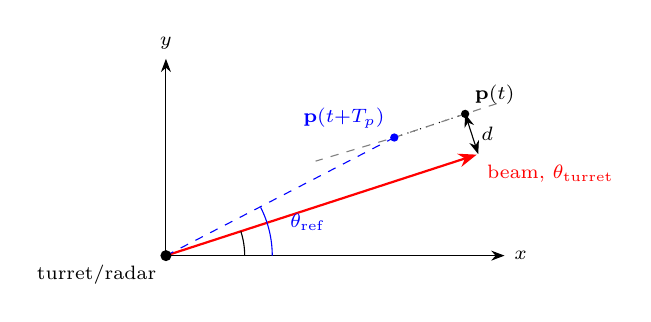
\begin{tikzpicture}[>=Stealth,font=\scriptsize]
\draw[->] (0,0) -- (4.3,0) node[right]{$x$};
\draw[->] (0,0) -- (0,2.5) node[above]{$y$};
\coordinate (O) at (0,0);
\coordinate (p) at (3.8,1.8);
\coordinate (pp) at (2.9,1.5);
\coordinate (B) at (18:4.15);
\coordinate (f) at ($(O)!(p)!(B)$);
\draw[thick,red,->] (O) -- (B) node[below right]{beam, $\theta_\mathrm{turret}$};
\draw[dashed,blue] (O) -- (pp);
\draw[dotted] (p) -- (pp);
\draw[gray,dashed] (4.2,1.93) -- (p) -- (pp) -- (1.9,1.2);
\fill (p) circle (1.5pt) node[above right]{$\vect p(t)$};
\fill[blue] (pp) circle (1.5pt) node[above left]{$\vect p(t{+}\Tp)$};
\draw[<->] (p) -- (f) node[midway,right]{$d$};
\draw (1.0,0) arc (0:18:1.0);
\draw[blue] (1.35,0) arc (0:27:1.35);
\node[blue] at (1.8,0.42) {$\theta_\mathrm{ref}$};
\fill (O) circle (2pt) node[below left]{turret/radar};
\end{tikzpicture}}
\caption{Elevation-plane geometry. The reference is the elevation of the predicted position $\vect p(t{+}\Tp)$; a hit is judged by the distance $d$ from the current target position to the beam.}
\label{fig:geom}
\end{figure}

%=====================================================================
\section{Mathematical Modeling}

\subsection{Target and radar models}

With the turret at the origin, $x$ horizontal and $y$ up, the target at $(x,y)$ has
\begin{equation}
r=\sqrt{x^2+y^2},\qquad \theta=\mathrm{atan2}(y,x).
\end{equation}
Radar samples at $t_k = k\,T_s$, $T_s=0.05$~s, are $r_m=r+n_r$, $\theta_m=\theta+n_\theta$ with zero-mean noise, $\sigma_r=1$~m and $\sigma_\theta=0.02^\circ=3.49\times10^{-4}$~rad.

The assignment does not give trajectories, so the following are our own engineering assumptions (in \texttt{target\_truth.m}). \emph{Scenario A:} $x=1800-100\,t$, $y=600$~m (speed 100~m/s). \emph{Scenario B:} A plus a smooth maneuver from $\tau=t-1\ge0$: an $x$ acceleration pulse $a_x=\tfrac{A_x}{2}\left(1-\cos\tfrac{2\pi\tau}{T_x}\right)$ for $0\le\tau\le T_x$, with $A_x=10$~m/s$^2$, $T_x=4$~s, and a lane change in $y$ made of a positive followed by a negative pulse of the same shape with $A_y=14$~m/s$^2$, $T_y=2.5$~s each. \emph{Scenario C:} identical trajectory to B, with \texttt{meas\_valid}$=0$ for $1.0\le t<1.5$~s (10 radar samples lost). The generator test confirms range $800$--$2000$~m, speed $\le150$~m/s, acceleration $\le20$~m/s$^2$ and elevation within the turret limits for all three.

\subsection{Target-state estimator}

The state is $\vect s=[x\;y\;v_x\;v_y\;a_x\;a_y]^T$ with a constant-acceleration model driven by white jerk of spectral density $q$ \cite{bs}. Over a step $\Delta t$,
\begin{equation}
\vect s_{k+1}=\vect F(\Delta t)\vect s_k,\quad
\vect F=\begin{bmatrix}I&\Delta t\,I&\tfrac12\Delta t^2I\\0&I&\Delta t\,I\\0&0&I\end{bmatrix},
\label{eq:F}
\end{equation}
\begin{equation}
P^-=\vect FP\vect F^T+\vect Q,\quad
\vect Q_{\rm axis}=q\begin{bmatrix}\frac{\Delta t^5}{20}&\frac{\Delta t^4}{8}&\frac{\Delta t^3}{6}\\[1pt]\frac{\Delta t^4}{8}&\frac{\Delta t^3}{3}&\frac{\Delta t^2}{2}\\[1pt]\frac{\Delta t^3}{6}&\frac{\Delta t^2}{2}&\Delta t\end{bmatrix},
\end{equation}
where $\vect Q_{\rm axis}$ acts on $(x,v_x,a_x)$ and on $(y,v_y,a_y)$ separately. The measurement is $\vect h(\vect s)=[\sqrt{x^2+y^2},\ \mathrm{atan2}(y,x)]^T$ with Jacobian
\begin{equation}
H=\begin{bmatrix}\frac{x}{r}&\frac{y}{r}&0&0&0&0\\[1pt]-\frac{y}{r^2}&\frac{x}{r^2}&0&0&0&0\end{bmatrix},\quad R=\mathrm{diag}(\sigma_r^2,\sigma_\theta^2).
\end{equation}
At a new valid measurement the update is
\begin{align}
\vect\nu&=\begin{bmatrix}r_m-\hat r\\ \mathrm{wrap}(\theta_m-\hat\theta)\end{bmatrix},\quad S=HP^-H^T+R,\nonumber\\
K&=P^-H^TS^{-1},\quad \hat{\vect s}=\hat{\vect s}^-+K\vect\nu,\\
P&=(I-KH)P^-(I-KH)^T+KRK^T,\nonumber
\end{align}
with $\mathrm{wrap}(a)=\mathrm{atan2}(\sin a,\cos a)$ keeping the angle innovation in $(-\pi,\pi]$ and the Joseph form keeping $P$ symmetric positive semidefinite. The filter is initialised on the first valid sample: position from $(r_m,\theta_m)$ with covariance $JRJ^T$ ($J$ the polar-to-Cartesian Jacobian), zero velocity and acceleration, and prior standard deviations $v_{\max}/2=75$~m/s and $a_{\max}/2=10$~m/s$^2$ per axis. The jerk density is $q=10$~m$^2$/s$^5$, fixed once for all scenarios. Its value is a fixed modelling choice that allows the filter to accommodate moderate departures from constant acceleration; The value $q=10$ was retained after comparing prediction-error
diagnostics for candidate values $q=1,3,10,30,100$..

The estimator is called at every 1~ms controller step and always performs the time update. The measurement update runs only if \texttt{meas\_valid} is true and the measurement is new. During a blackout it therefore propagates $(\hat{\vect s},P)$ open loop and $P$ grows through $\vect Q$.

\subsection{Predictor and reference}

The predictor applies Eq.~\eqref{eq:F} with $\Delta t=\Tp=0.5$~s to the current estimate and adds $\vect Q(\Tp)$ to the covariance, then converts position to elevation:
\begin{equation}
\hat{\vect s}_p=\vect F(\Tp)\hat{\vect s},\quad
\theta_p=\mathrm{atan2}(y_p,x_p),\quad r_p=\sqrt{x_p^2+y_p^2},
\end{equation}
\begin{equation}
\theta_\mathrm{ref}=\min\{\max\{\theta_p,\,-10^\circ\},\,85^\circ\}.
\end{equation}
The clamp enforces the turret limits through the reference (the plant has no end stops).

\subsection{Turret elevation plant}

With $J_\mathrm{eq}=J_\mathrm{turret}+N^2J_m=3200$~kg\,m$^2$ (rotor inertia reflected through $N=100$), the equations implemented in \texttt{turret\_plant.m} are
\begin{align}
J_\mathrm{eq}\ddot\theta&=NK_t\,i-b\,\dot\theta,\\
L_m\dot i&=V_m-R_m i-NK_e\dot\theta.
\end{align}
Taking Laplace transforms and eliminating $i$,
\begin{align}
G_p(s)&=\frac{\Theta}{V_m}=\frac{NK_t}{s\,D(s)}=\frac{1000}{s\,(320s^2+3350s+1\,001\,500)},\label{eq:Gp}\\
D(s)&=L_mJ_\mathrm{eq}s^2+(L_mb+R_mJ_\mathrm{eq})s+R_mb+N^2K_tK_e.\nonumber
\end{align}
Eq.~\eqref{eq:Gp} was checked against the coefficients computed in \texttt{params.m}. The model is linear and assumes an ideal gear, viscous friction only on the turret side, and no gravity, unbalance, backlash or saturation. The open-loop poles are $0$ and $-5.23\pm j55.7$~rad/s. The low-frequency velocity constant is $\Kv=1000/1\,001\,500=9.985\times10^{-4}$~rad/s per V.

%=====================================================================
\section{Controller Design and Analysis}\label{sec:ctrl}

\subsection{Gain selection}

$G_p$ has one integrator, so $\Kp G_p$ is type~1 and the loop for a ramp reference of rate $\omega$ has steady error $\omega/(\Kp\Kv)$, i.e.\ the output lags the reference by $1/(\Kp\Kv)$~s. The reference is the prediction of $\theta(t+\Tp)$. Choosing
\begin{equation}
\Kp=\frac{1}{\Tp\Kv}=2003.0\ \mathrm{V/rad}
\end{equation}
makes the lag exactly $\Tp$, so for a constant line-of-sight rate the turret points at $\theta(t)$, the same angle at which the target is when the pulse is judged. A larger gain would shrink the lag below $\Tp$ and make the turret \emph{lead} the target, which is not useful, and it also moves toward the stability limit below. The result also gives a loop gain $\Kp G_p\approx 1/(\Tp s)$ at low frequency, i.e.\ a gain crossover near $1/\Tp = 2$~rad/s, far below the 55.7~rad/s electromechanical mode and the radar sampling angular frequency of approximately
125.7~rad/s (corresponding to a Nyquist angular frequency
of 62.8~rad/s).

\subsection{Stability}

The closed-loop characteristic polynomial is
\begin{equation}
320s^3+3350s^2+1\,001\,500\,s+1000\,\Kp=0.
\end{equation}
The Routh array has first column $320,\ 3350,\ (3350\cdot1\,001\,500-320\cdot1000\Kp)/3350,\ 1000\Kp$, so stability requires
\begin{equation}
0<\Kp<\frac{3350\cdot1\,001\,500}{320\,000}=10\,484.45\ \mathrm{V/rad}.
\end{equation}
Our $\Kp=2003$ lies inside this range. The closed-loop poles are $-4.229\pm j55.631$ and $-2.011$, all in the left half-plane. The sum of poles ($-10.469$) matches $-3350/320$. Table~\ref{tab:lin} lists margins and the step response (0.3~rad, real plant in the loop, RK4, 1~ms).

\begin{table}[t]
\caption{Linear loop results ($\Kp=2003$ V/rad)}
\label{tab:lin}
\centering\footnotesize
\begin{tabular}{lc}
\toprule
Quantity & Value\\
\midrule
Phase margin & $89.62^\circ$\\
Gain margin & $5.234$ ($14.38$ dB)\\
Step final value / overshoot & $0.30000$ rad / $0\%$\\
10--90\% rise time, 2\% settling time & $1.090$ s, $1.946$ s\\
Ramp steady-state lag (simulated / $1/(\Kp\Kv)$) & $0.5000$ s / $0.5000$ s\\
\bottomrule
\end{tabular}
\end{table}

The dominant real pole $-2.011$ (time constant $\approx0.50$~s) explains the step response: the lightly damped pair at $-4.2\pm j55.6$ decays about twice as fast and the step shows no overshoot. The turret closed-loop bandwidth of roughly 2~rad/s also low-pass filters the radar noise that survives the estimator and prediction.

\subsection{Limits of the lag compensation}

Writing $T(s)=1/(1+c_1s+c_2s^2+c_3s^3)$ with $c_1=G_{d3}/(G_{n}\Kp)=0.5$, $c_2=G_{d2}/(G_n\Kp)=1.6725\times10^{-3}$ ($G_{d\cdot}$, $G_n$ the denominator and numerator coefficients of $G_p$), the pointing error for the reference $\theta(t+\Tp)$ is, to second order in $s$,
\begin{equation}
\begin{gathered}
\theta-\theta(t)\approx\left[(\Tp-c_1)s+c\,s^2\right]\theta,\\
c=\tfrac{\Tp^2}{2}-c_1\Tp+c_1^2-c_2=0.1233\ \mathrm{s^2}.
\end{gathered}
\end{equation}
The velocity term vanishes since $c_1=\Tp$, but a constant angular acceleration $\ddot\theta$ leaves an error $c\,\ddot\theta$. The simulation with $\ddot\theta=0.020$~rad/s$^2$ gave $2.462\times10^{-3}$~rad against $c\ddot\theta=2.466\times10^{-3}$~rad. At a range of 1~km this is about 2.5~m, larger than $R_\mathrm{eng}$. Hence the compensation is exact only for constant line-of-sight rate in steady state. Maneuver onset, initial slew, measurement recovery and angular acceleration (which is non-zero even for a straight-line target) are not cancelled.

\subsection{Firing logic}

The firing logic is separate from $V_m$ and uses the estimated present position $\hat{\vect p}=(\hat x,\hat y)$. With beam direction $\vect u=[\cos\theta_t,\sin\theta_t]^T$ and normal $\vect n=[-\sin\theta_t,\cos\theta_t]^T$,
\begin{equation}
\hat d=|\vect n^T\hat{\vect p}|,\quad
\sigma_\perp=\sqrt{\vect n^TP_{xy}\vect n},
\end{equation}
and the gate opens only if $\vect u^T\hat{\vect p}>0$ (target in front of the turret; otherwise the closest beam point is the origin) and $\hat d+k_\sigma\sigma_\perp\le R_\mathrm{eng}=2$~m with $k_\sigma=1$. The $\sigma_\perp$ term makes the gate conservative when the estimate is uncertain. A pulse is issued when the gate is open, at least $1\,\mathrm{s}+10^{-6}\,\mathrm{s}$ (round-off guard) has passed since the last pulse, and \texttt{fire\_cmd} was low on the previous step. \texttt{fire\_cmd} is high for exactly one step, so each pulse is a clean $0\to1$ transition.

An \emph{issued pulse} is not a \emph{successful engagement}. The gate uses the estimate $\hat{\vect p}$ and the measured turret angle, whereas success depends on the true target position at the firing instant, so estimation error and the residual pointing error above can turn an issued pulse into a miss.

%=====================================================================
\section{Simulation and Results}

\subsection{Setup}

The closed-loop test (\texttt{test\_turret\_controller.m}) uses a fixed 1~ms step over $0\le t\le10$~s, RK4 integration of \texttt{turret\_plant} (states $\theta,\dot\theta,i$, all initially zero), and a zero-order hold on $V_m$ over each step. The radar provides a new sample every 50~ms. A pulse lasts one step and is judged at the step where \texttt{fire\_cmd} goes $0\to1$, using the true target position and the turret angle at that step; a hit means distance to the beam ray $\le2$~m. The controller never calls ground truth, which the test checks by scanning the controller, estimator and predictor code. Metrics after $t=3$~s are used since the turret starts at $0$~rad and slews to about $18^\circ$ initially. Predicted-elevation error is $(\theta_p-\theta(t{+}\Tp))\,r$ in metres for $t\ge1$~s.

% ---- Figures 1 and 2: target truth and radar measurements side by side ----
\begin{figure*}[t]
\centering

\begin{minipage}[t]{0.48\textwidth}
    \centering
    \figbox{tmg_fig1_truth}{1.5in}
    \caption{Ground-truth target trajectories and constraint verification for Scenarios A, B and C. The plots show the elevation-plane trajectory, range, elevation, speed, acceleration and radar measurement validity. Scenarios B and C have identical target motion; Scenario C differs only through the radar blackout.}
    \label{fig:truth}
\end{minipage}
\hfill
\begin{minipage}[t]{0.48\textwidth}
    \centering
    \figbox{tmg_fig2_measurements}{1.5in}
    \caption{Radar measurement validation for Scenario C. The plots compare true and measured range and elevation around the 0.5~s blackout from 1.0 to 1.5~s. Red crosses indicate missing measurements. The histograms show the range and elevation noise distributions, with measured standard deviations of 0.995~m and 0.02006$^\circ$.}
    \label{fig:measurements}
\end{minipage}

\end{figure*}

\begin{table}[t]
\caption{Closed-loop results (own simulation, 10 s)}
\label{tab:res}
\centering\footnotesize
\begin{tabular}{lccc}
\toprule
 & A & B & C\\
\midrule
Pulses issued / hits & 8 / 8 & 7 / 5 & 7 / 5\\
First successful hit [s] & 2.700 & 4.200 & 4.130\\
Miss RMS, $t\ge3$ s [m] & 0.77 & 1.21 & 1.19\\
Miss max, $t\ge3$ s [m] & 1.27 & 2.62 & 2.54\\
Time within 2 m, $t\ge3$ s & 100\% & 90.2\% & 90.5\%\\
Pred.\ elevation RMS err. [m] & 0.74 & 1.82 & 1.77\\
Peak $|V_m|$ [V] / peak $|i|$ [A] & 645 / 101 & 645 / 101 & 645 / 101\\
\bottomrule
\end{tabular}
\end{table}

\subsection{Scenario comparison}

The target trajectories and radar measurements are validated in Figs.~\ref{fig:truth} and~\ref{fig:measurements}. Table~\ref{tab:res} and Figs.~\ref{fig:elev}--\ref{fig:miss} summarise the closed-loop tracking and engagement performance.

In A every pulse hit and the beam stayed within 2~m of the target after 3~s, with 0.77~m RMS miss. This residual comes from estimation noise and from the non-zero line-of-sight acceleration of a straight-line target. We did not separate the two contributions.

In B and C the maneuver (nominally $1\le t\lesssim5$ s in $x$ and $\lesssim6$ s in $y$ under our trajectory) overlaps the evaluation window, so the miss RMS and maximum are about 1.6 and 2.1 times those of A and the prediction error is roughly 2.4 times larger. This is consistent with the constant-acceleration predictor being driven away from its model by the changing acceleration, together with the uncancelled $c\ddot\theta$ term of Section~IV-C. Two of the seven pulses missed in each of B and C, and the first successful hit moved from 2.70~s to about 4.2~s. B and C are close, so the 0.5~s blackout had little visible effect on these aggregate metrics. All three scenarios therefore achieved interception success by our own scoring, but with markedly less margin in the maneuvering cases (maximum miss $\approx2.6$~m against the 2~m radius).

\begin{figure}[t]
\centering
\figbox{fig1_elevation_tracking}{2.6in}
\caption{True elevation, reference $\theta_\mathrm{ref}$ (prediction at $t+\Tp$), turret angle and pulses (hits and misses) for A, B, C.}
\label{fig:elev}
\end{figure}

\begin{figure}[t]
\centering
\figbox{fig2_pointing_miss}{2.6in}
\caption{True beam-to-target distance with the 2~m threshold (dashed) and issued pulses.}
\label{fig:miss}
\end{figure}

\subsection{Radar blackout (Scenario C)}

Ten samples between 1.00 and 1.45~s are lost, leaving 191 valid updates. The estimator's update counter stayed at 20 throughout the blackout and went to 21 at 1.50~s. During this interval the filter only performs the time update, since no new information exists and a correction with a stale or missing measurement would corrupt the state. The predictor keeps extrapolating from the last estimate with constant acceleration, so $\theta_\mathrm{ref}$ and $V_m$ stay continuous; the largest voltage step in the blackout was 0.16~V. The price is uncertainty: $\sigma_\perp$ rose from 0.38~m to 1.91~m. Because the gate requires $\hat d+\sigma_\perp\le2$~m, at $\sigma_\perp=1.91$~m it can open only when $\hat d<0.09$~m, so firing is effectively suppressed near the end of the blackout. The target also keeps maneuvering unobserved, so the estimate drifts from the truth. Fig.~\ref{fig:black} plots the reference, $\sigma_\perp$ and the gate quantity across the blackout, so that growth and recovery of the uncertainty after 1.5~s can be read directly. The blackout does have an effect on prediction and uncertainty; the test only shows that it did not cause loss of the filter or discontinuity in the command.

\subsection{Control effort and limitations}

The peak voltage is 645~V and the peak current 101~A in all three scenarios, both in the initial slew: $\Kp\,\theta_\mathrm{ref}(0)=2003\times0.322\approx645$~V, since $\theta_\mathrm{ref}(0)\approx18.4^\circ$ and the turret starts at 0. After the slew the peak voltage is 106.5--106.9~V. The turret angle remained between $0$ and a maximum of 34.44--36.94$^\circ$ across the scenarios, inside $-10^\circ$ to $85^\circ$. \textbf{The simulation does not model voltage or current saturation}, nor motor or amplifier ratings, so these figures are demands of an ideal linear drive and have not been checked against any hardware limit. A saturating drive would change the initial slew; we did not simulate this, so its effect on the first engagement is unknown.

The time histories of the control voltage, motor current and turret response are shown in Fig.~\ref{fig:control}.

% ---- Figure 3: control effort ----
\begin{figure*}[t]
\centering
\figbox{fig3_control_effort}{3.0in}
\caption{Control effort and turret response during closed-loop tracking. The figure shows the control and actuator response associated with the initial turret slew and subsequent target tracking. The large initial demand corresponds to the initial slew from the zero-degree turret position. No voltage or current saturation is included in the plant model.}
\label{fig:control}
\end{figure*}

The linear loop response is in Fig.~\ref{fig:lin}.

% ---- Figures 7 and 9: blackout zoom and linear loop analysis side by side ----
\begin{figure*}[t]
\centering

\begin{minipage}[t]{0.48\textwidth}
    \centering
    \figbox{fig4_blackout_zoom}{2.4in}
    \caption{Scenario C, $0.8$--$2.2$~s: predicted reference (C and B), cross-beam uncertainty $\sigma_\perp$ and gate quantity $\hat d+\sigma_\perp$. Shaded region is the blackout.}
    \label{fig:black}
\end{minipage}
\hfill
\begin{minipage}[t]{0.48\textwidth}
    \centering
    \figbox{fig5_linear_loop}{2.4in}
    \caption{Linear loop analysis with $\Kp=2003$ V/rad: Bode plot of $\Kp G_p$, 0.3~rad step response and ramp error (real \texttt{turret\_plant}).}
    \label{fig:lin}
\end{minipage}

\end{figure*}

%=====================================================================
\section{Final Evaluation}\label{sec:final}

\textbf{The instructor's evaluation has not yet been run.} It requires an evaluation script and cases that were not available when this report was prepared. No instructor result, score or case is therefore reported, and none of the results in Section~V should be read as one. The scenarios in Section~V use trajectories that we defined ourselves.

What \emph{has} been done is our own validation. The controller test passed 78/78 structural/design checks (file availability, gain, Routh bound, poles and margins, step/ramp/acceleration tracking, estimator initialisation, pulse and recharge behaviour, uncertainty gate, absence of ground-truth calls, closed-loop scenarios, blackout handling and turret angle-limit behaviour) and 6/6 performance flags. The target-generator test passed 63/63 checks and the estimator test 47/47. These tests show consistency between the code and the models in this report; they do not demonstrate performance on unseen maneuvers. Interception success is defined as at least one hit among issued pulses and interception time as the first hit \cite{assign}; the evaluation cases may use different maneuvers and blackout timing, and the estimator, predictor and controller will be used unchanged.

We expect the fixed constant-acceleration model, $q$ and the gate threshold to be the main factors determining generalisation, because Scenarios B and C already show reduced margin during maneuvering. This is an expectation based on our results, not a verified outcome. [\emph{These expectations remain to be verified using the instructor's
evaluation cases.}]

%=====================================================================
\section{Conclusions}

An EKF with a constant-acceleration model, a 0.5~s Cartesian prediction, and a single proportional gain $\Kp=1/(\Tp\Kv)=2003$~V/rad form a simple, analytically supported predictive-feedback design. The loop is stable with $89.6^\circ$ phase margin and gain margin 5.23, and its ramp lag equals the prediction horizon. In our own simulations all three scenarios produced at least one hit, with all 8 pulses hitting in the non-maneuvering case and 5 of 7 in each maneuvering case. The main limitations are: (i) the compensation is not exact under angular acceleration, so accuracy drops during maneuvers; (ii) the uncertainty-aware gate suppresses firing during and shortly after a blackout; (iii) saturation and hardware limits are not modelled, and the initial-slew demands of 645~V and 101~A are therefore unvalidated; (iv) the scenario trajectories are our own assumptions; and (v) the instructor evaluation is still pending.

\begin{thebibliography}{1}
\bibitem{assign} P. Agarwal, ``Assignment 2: Mumbai 2044 -- Predictive tracking and turret control for a maneuvering aerial target,'' ME319 Control Systems, IIT Bombay, Autumn 2026.
\bibitem{bs} Y. Bar-Shalom, X. R. Li, and T. Kirubarajan, \emph{Estimation with Applications to Tracking and Navigation}. New York, NY, USA: Wiley, 2001.
\end{thebibliography}

%=====================================================================
%=====================================================================
%=====================================================================
\clearpage
\onecolumn
\section*{Appendix: Use of AI and Computational Tools}

\textbf{Tools used.}
MATLAB was used for implementation, numerical simulation, testing and
generation of plots. ChatGPT and Claude were used as AI-assisted tools
during the development and documentation of the assignment.

\textbf{Nature of AI assistance.}
AI assistance was used to help develop and review parts of the MATLAB
implementation, including the target-motion model, state-estimation
approach, prediction logic, controller implementation and test
procedures. AI assistance was also used to organise the technical
explanation, derive and check mathematical expressions, and prepare
the \LaTeX{} report.

The final implementation, simulation runs, test execution, interpretation
of numerical results and preparation of the submission were carried out
and reviewed by the author.

\textbf{Accepted, modified and rejected suggestions.}
AI-generated suggestions were treated as proposals rather than
automatically accepted results. The proposed estimation and prediction
approach was checked against the assignment requirements and tested
using the MATLAB implementation. Controller gains and stability
conditions were checked against the derived plant model. Suggestions
that were inconsistent with the plant equations, assignment constraints
or observed simulation behaviour were not retained.

The proportional gain was selected analytically using the plant
velocity constant and the specified prediction horizon, rather than
being accepted solely from an AI-generated numerical recommendation.
The firing logic, measurement blackout handling and pulse-spacing
behaviour were also checked through dedicated test cases.

\textbf{Independent validation.}
MATLAB test scripts were used to validate the plant, target generator,
estimator, predictor and controller. The plant coefficients, equivalent
inertia, controller gain, Routh stability bound, closed-loop poles and
tracking results were checked against the mathematical model.
The controller test reported 78/78 structural and design checks and
6/6 performance flags; the target-generator and estimator tests
reported 63/63 and 47/47 checks, respectively.

The closed-loop results presented in this report are taken from the
MATLAB simulation output. The instructor's final evaluation has not
been performed, and no official evaluation result is claimed.

AI assistance was used to support the work, but the author reviewed
the implementation, checked the mathematical reasoning and remains
responsible for the submitted code, results and conclusions.

\end{document}